% 79-45(79쪽) — $\seg{AB}$ 를 지름으로 하는 원 $O$ 와 원 위의 점 $\pt{C}$(원문 「오른쪽 그림」). 스캔 화질이 낮아 TikZ 로 다시 그림.
% 라벨은 원문 것만: 점 이름 A·B·C·O, 변의 길이 $2$·$\sqrt{5}$, 각 $\alpha$·$\beta$.
% $\sin(2\alpha+\beta)$(답)가 그림에서 읽히지 않게 각도·눈금은 적지 않는다.
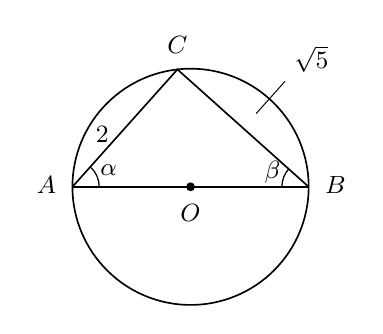
\begin{tikzpicture}[line width=0.6pt, x=1cm, y=1cm]
  \draw (0,0) circle (1.5);
  \draw (-1.5,0) -- (1.5,0);
  \draw (-1.5,0) -- (-0.1667,1.4907) -- (1.5,0);
  \fill (0,0) circle (1.6pt);
  \draw[line width=0.45pt] (-1.5,0) ++(0:0.34) arc (0:48.2:0.34);
  \draw[line width=0.45pt] (1.5,0) ++(180:0.34) arc (180:138.2:0.34);
  \draw[line width=0.35pt] (0.834,0.931) -- (1.20,1.34);
  \node[font=\small] at (-1.04,0.21) {$\alpha$};
  \node[font=\small] at (1.04,0.19) {$\beta$};
  \node[font=\small] at (-1.12,0.67) {$2$};
  \node[font=\small, anchor=south west] at (1.19,1.33) {$\sqrt{5}$};
  \node[font=\small, anchor=east] at (-1.58,0.02) {$\pt{A}$};
  \node[font=\small, anchor=west] at (1.58,0.02) {$\pt{B}$};
  \node[font=\small, anchor=north] at (0,-0.10) {$\pt{O}$};
  \node[font=\small, anchor=south] at (-0.1667,1.56) {$\pt{C}$};
\end{tikzpicture}
